\begin{prob}
    Suppose a BFS is run on the graph below using node 1 as the source node. Which
    node will be the BFS predecessor of node 9? You should use the convention that neighbors
    are produced in ascending order by label.

    \begin{center}
        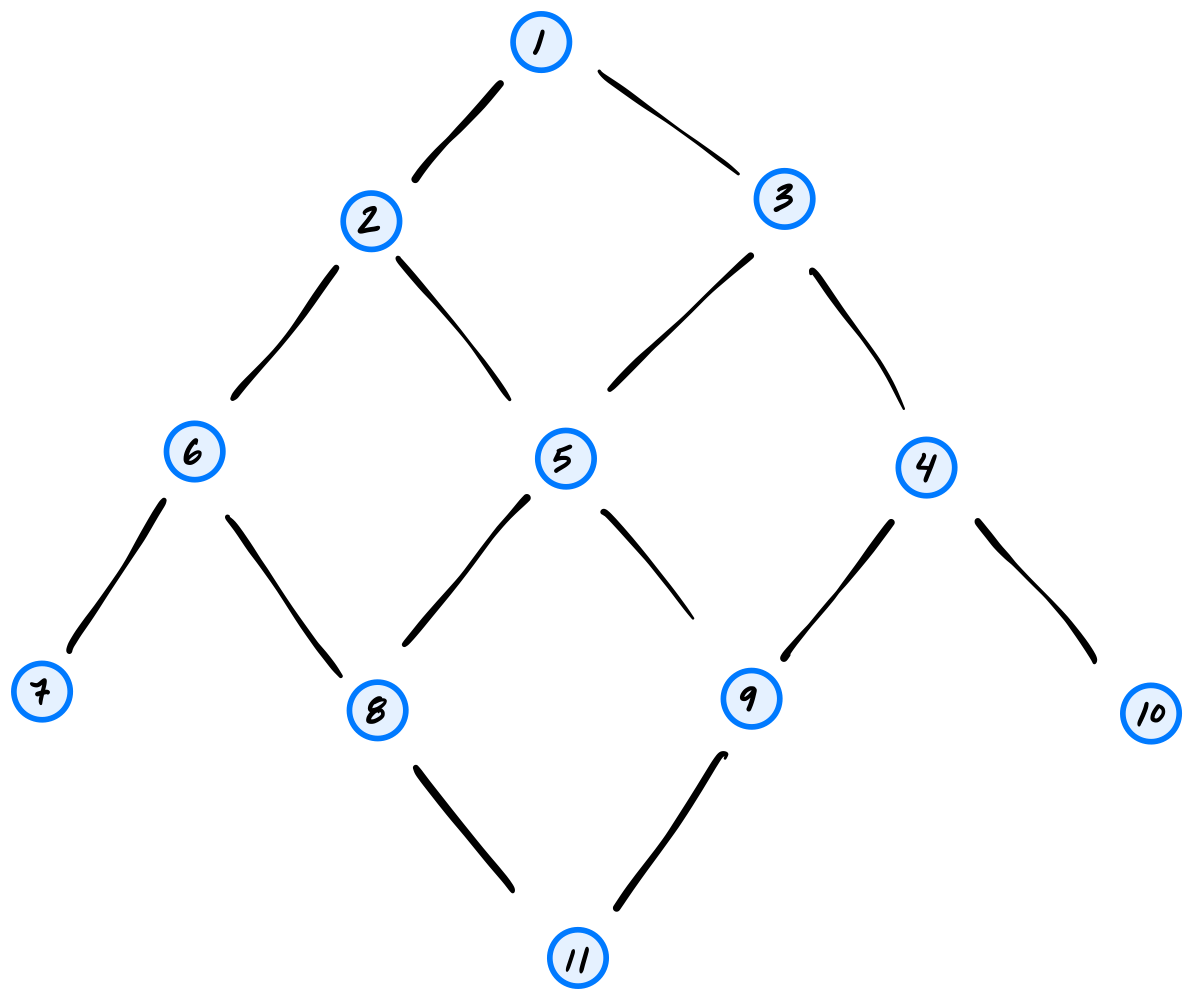
\includegraphics[width=.6\textwidth]{./fig/g2.png}
    \end{center}

    \inlineresponsebox[1.5in]{5}

\end{prob}
